%%%%%%%%%%%%%%%%%%%%%%%%%%%%%%%%%%%%%%%%%%%%%%%%%%%%%%%%%%%%%%%%%%%%%%%%%%%%
%% Author template for Management Science (mnsc) for articles with e-companion (EC)
%% Mirko Janc, Ph.D., INFORMS, mirko.janc@informs.org
%% ver. 0.95, December 2010
%%%%%%%%%%%%%%%%%%%%%%%%%%%%%%%%%%%%%%%%%%%%%%%%%%%%%%%%%%%%%%%%%%%%%%%%%%%%
\documentclass[mnsc,blindrev]{informs3} % current default for manuscript submission
%\documentclass[mnsc,nonblindrev]{informs3}

\OneAndAHalfSpacedXI % current default line spacing
%%\OneAndAHalfSpacedXII 
%%\DoubleSpacedXII
%%\DoubleSpacedXI

% If hyperref is used, dvi-to-ps driver of choice must be declared as
%   an additional option to the \documentstyle. For example
%\documentclass[dvips,mnsc]{informs3}      % if dvips is used
%\documentclass[dvipsone,mnsc]{informs3}   % if dvipsone is used, etc.

% Private macros here (check that there is no clash with the style)
\usepackage{graphicx}

% Natbib setup for author-year style
\usepackage{natbib}
 \bibpunct[, ]{(}{)}{,}{a}{}{,}%
 \def\bibfont{\small}%
 \def\bibsep{\smallskipamount}%
 \def\bibhang{24pt}%
 \def\newblock{\ }%
 \def\BIBand{and}%

%% Setup of theorem styles. Outcomment only one.
%% Preferred default is the first option.
\TheoremsNumberedThrough     % Preferred (Theorem 1, Lemma 1, Theorem 2)
%\TheoremsNumberedByChapter  % (Theorem 1.1, Lema 1.1, Theorem 1.2)
\ECRepeatTheorems

%% Setup of the equation numbering system. Outcomment only one.
%% Preferred default is the first option.
\EquationsNumberedThrough    % Default: (1), (2), ...
%\EquationsNumberedBySection % (1.1), (1.2), ...

% For new submissions, leave this number blank.
% For revisions, input the manuscript number assigned by the on-line
% system along with a suffix ".Rx" where x is the revision number.
\MANUSCRIPTNO{}

%%%%%%%%%%%%%%%%
\begin{document}
%%%%%%%%%%%%%%%%

% Outcomment only when entries are known. Otherwise leave as is and
%   default values will be used.
%\setcounter{page}{1}
%\VOLUME{00}%
%\NO{0}%
%\MONTH{Xxxxx}% (month or a similar seasonal id)
%\YEAR{0000}% e.g., 2005
%\FIRSTPAGE{000}%
%\LASTPAGE{000}%
%\SHORTYEAR{00}% shortened year (two-digit)
%\ISSUE{0000} %
%\LONGFIRSTPAGE{0001} %
%\DOI{10.1287/xxxx.0000.0000}%

% Author's names for the running heads
% Sample depending on the number of authors;
% \RUNAUTHOR{Jones}
% \RUNAUTHOR{Jones and Wilson}
% \RUNAUTHOR{Jones, Miller, and Wilson}
% \RUNAUTHOR{Jones et al.} % for four or more authors
% Enter authors following the given pattern:
%\RUNAUTHOR{}

% Title or shortened title suitable for running heads. Sample:
% \RUNTITLE{Bundling Information Goods of Decreasing Value}
% Enter the (shortened) title:
\RUNTITLE{Signal and Noise of Reviews}

% Full title. Sample:
% \TITLE{Bundling Information Goods of Decreasing Value}
% Enter the full title:
\TITLE{The Signal and Noise of Performance Reviews in an Online Market Place: The Case of Residential Solar Installations}

% Block of authors and their affiliations starts here:
% NOTE: Authors with same affiliation, if the order of authors allows,
%   should be entered in ONE field, separated by a comma.
%   \EMAIL field can be repeated if more than one author
\ARTICLEAUTHORS{%
\AUTHOR{Snidely Slippery}
\AFF{Department of Bread Spread Engineering, Dairy University, Cowtown, IL 60208, \EMAIL{slippery@dairy.edu}} %, \URL{}}
\AUTHOR{Marg Arinella}
\AFF{Institute for Food Adulteration, University of Food Plains, Food Plains, MN 55599, \EMAIL{m.arinella@adult.ufp.edu}}
% Enter all authors
} % end of the block

\ABSTRACT{%
This paper  
% Enter your abstract
}%

% Sample
%\KEYWORDS{deterministic inventory theory; infinite linear programming duality;
%  existence of optimal policies; semi-Markov decision process; cyclic schedule}

% Fill in data. If unknown, outcomment the field
\KEYWORDS{marketplace, reviews} \HISTORY{Update: November, 2019}

\maketitle
%%%%%%%%%%%%%%%%%%%%%%%%%%%%%%%%%%%%%%%%%%%%%%%%%%%%%%%%%%%%%%%%%%%%%%

% Samples of sectioning (and labeling) in MNSC
% NOTE: (1) \section and \subsection do NOT end with a period
%       (2) \subsubsection and lower need end punctuation
%       (3) capitalization is as shown (title style).
%
%\section{Introduction.}\label{intro} %%1.
%\subsection{Duality and the Classical EOQ Problem.}\label{class-EOQ} %% 1.1.
%\subsection{Outline.}\label{outline1} %% 1.2.
%\subsubsection{Cyclic Schedules for the General Deterministic SMDP.}
%  \label{cyclic-schedules} %% 1.2.1
%\section{Problem Description.}\label{problemdescription} %% 2.

% Text of your paper here

\section{Introduction}

Increasing adoption of rooftop solar panels ( Recent statatistics from EIA)

Residential solar PV capacity increased by 300\%  in last ....year (REFERENCE)

Online marketplaces is an innovative way/ business model  to boost the rooftop solar panel adoption as (Information sharing becomes easier)...
There is an increasing trend of installing rooftop panels through online market places. Give specific statistics,  Residential solar PV installations through online platforms increased by ....  in last ....year (REFERENCE)

Online reviews are essential part of the customer experience in platforms. In fact, there are studies that show that reviews have significant impact on customers'  decision making process.  (See, e.g., CITE THE PAPERS  that provide evidence in the context of  BLAH)


In the literature, there are papers that show the positive impact of reviews on sales. There are also other papers that demonstrate  (AVERAGE LIT)

In this paper, different from this literature, our primary goal is to study the impact of dispersion of ratings on the  performance metric of the platform, which is a composite of many firms. To the best of our knowledge, there is no prior work that has studied this. 

Our paper is also related to papers that investigates the effect of ratings on a single firm's performance metrics. In that stream, there is no consensus about the ultimate impact of dispersion of ratings on the firm's performance metric. [POSITIVE IMPACT]  AND [NEGATIVE IMPACT]

Different from these papers, we took a marketplace perspective, and ....

Our objective is to understand the impact of review dispersion on the activity level of each participating supplier on the platform, which has not been studied before.



\section{Literature and Theory Development }
 \begin{hypothesis}
There is a U-Shaped relationship between the \textbf{variation of reviews} and installers' activity intensity. 
\end{hypothesis}

 \begin{hypothesis}
There is a U-Shaped relationship between the \textbf{variation of reviews on a market} and the market activity intensity. 
\end{hypothesis}
\section{Data and Settings}
\subsection{Market Place}
Our analysis are based off the activities on an online marketplace(MKT) for resident solar. MKT is an independent comparison shopping website that provided consumers an outlet for shopping for solar installations. The website provides consumers with access to hundreds of vetted solar installers as well as information about solar technologies and solutions. 

\paragraph{How MKT works:}
1. Customers visit MKT website and enter their property address along with other details.  \\
2. Marketplace informs the installer the arrival of customer along with customer's requirement and preferences. \\
3. Installers decide to make a customized proposal the the customer. This is called place a bid. \\
4. The customer may proceed and choose one installer(a match is successfully made) or give up this process(go for another offline option, or give up on installing solar for the moment) \\ 
We obtained a rich panel of MKT data with all its vetted installers, installers' monthly action and performance(bids made and bids won) and all its reviews(text content and ratings) from the beginning of the platform to April of 2018. 

\subsection{Installers}
Solar Installers decision on the platform: 

\begin{enumerate}
\item  \textbf{Join}. Join the platform. It is worth noting that the marketplace actively reach out to solar installers to recruit them to join to platform and help them set up the website. So unlike physical businesses, the fixed cost of entry is low. Thus, the process of joining the platform is not the focus of this study.( ADD REFERENCE , something about barrier of entry = 0)  \\
\item  \textbf{Active and put in efforts}. Actively monitor the platform and make bids to attract customer. We are interested in the\textit{ intensity of efforts}, which is measured by how many proposals that an installer makes per month.(FIND REFERENCE THAT THIS TAKES TIME AND EFFORT; IS THE ESSENTIAL DECISION)\\
\end{enumerate}

Lastly, we don't observe quitting the platform the same way as physical store closes off. We simply observe inactive profiles. 


\subsection{Customers}
Customers will join the platform, provide the basic infos including their property details. They will receive installer proposals. If the customer ended up working with the installer, they will have an opportunity to leave a review. \\
The platform verifies the customer who left reviews. So we can treat reviews as authentic and not manipulated. 

\subsection{Summary Statistics}
In the merged dataset, we have a installer-month level panel dataset that depicted installers' actions. The dataset features: 
\begin{itemize}
\item Solar installers: 416 different installers
\item Time period: from 2013 to 2018
\item Ratings and reviews: 3607 pieces of review records with the rating, text content, timestamp, and the installer that is associated  
\end{itemize}
\subsection{Defining Local Market} 
Solar installers are in essence competing on a number of local markets with adjacent installers.  This is due to these characteristics of solar installations: sollar installation is a combination of product and service; the service component requires installers' multiple visits to the customer site;  customers tend to only seek out local installers and installers tend to only compete locally. This is also reflected in MKT's setting- installers specify a service region; installers will only be notified of customer arrival and act on the lead if the customer falls into that region. Customer also sees installer's distance to their locations and might factor that in their decision. Thus, we want to create a distance and density based \textit{clusters} that reflect the local competition feature. 
We also do not want to simply use state of county boarder because it was quite common for installers to cross county and state lines to serve customers. Instead, we create local market geographic division following the following steps: 
\begin{enumerate}
	\item First, for every MKT installer, we determine its location using the 5-digit zip code they listed and the representative coordinates of that Zipcode based on data provided by the US Census(https://www.census.gov/geo/maps-data/data/gazetteer.html). 
	\item  We run a location and density based clustering algorithm(OBTICS, more details below) to cluster the pool of nationwide installers into clusters, which we later refer to as "markets".  Ordering points to identify the clustering structure (OPTICS) is an algorithm for finding density-based clusters in spatial data.  We set the radius to be 50 miles(can change) and arrived at X clusters, each cluster contains X to X installers. We use this cluster to define our market boundary geographically.   
	\item we used parameters X and X for OPTICS algorithm after we performed grid search on the parameters from X to X. We use Calinski-Harabasz index to evaluate the clustering parameter and choose the parameter that optimized the Calinski-Harabasz index, while also reflected the reality on the ground that installer usually install locally ( within 1.5hrs of driving distance).
\end{enumerate}
The figure X and X illustrated the geographic distribution of all installers in the dataset ( left) and the centroid of local markets after OPTICS clustering(right). 

\subsubsection{Market Condition}
Once the algorithm gave us the clusters that defines market divisions, we augment the data with Tracking The Sun data to capture local market conditions. The goal of incorporating Offline Market Characteristics is to capture both installer and customer' outside options. We use the same Market definition from DBSCAN clustering and computed the following aggregate level variables: 
\begin{enumerate}
	\item Market Revenue: the sum of all solar installations within that market during a month. The market revenue variable measures the total opportunities of solar installations on that market. 
\end{enumerate} 
\section{Model and Measures}
\textbf{Overviews}: first we introduce the key DV, dispersion of the reviews. Then we take a look at the impact of the key DV on individual firm level; then we look at the impact of dispersion on platform level in section XX.  

\subsection{Measure Reviews Dispersion}
Define dispersion. Give examples. 
Independent Variable: Entropy of Reviews Rating
We use entropy as the independent variable of interests. Entropy is a common measure in information theory. We use entropy to capture the information content in raviews' rating. \\ 
Following the following formula:  \\ 
\begin{equation}
H(X)=-\sum P(X)log(1/P(x)))
\end{equation}

For every installers, we calculate entropy on two scopes: \\
1. Entropy on own reviews, denote as $ENT_{self}$ \\ 
2. Entropy on peer installers' reviews, denote as $ENT_{others}$ \\
\subsection{Installer Level Analysis}

\subsubsection{Dependent Variable: Installer Activity Level}
We use quotes given to proxy the intensity of activities. 
 \subsubsection{Control Variables\\} 
\textbf{Price}:   $PriceDiff_{i,t}$: we use Tracking the Sun data to find the installers' prices. We first find the unit price: price per KW. Price per KW is a common way to assess the price level of a solar system, as the final price tag of the solar system will be dependent on the size. We then compute the variable$PriceDiff_{i,t}$ as the difference in unit price between installer and the average unit price of their competitors on the local market. \\
\textbf{Average Reviews}: the average reviews of installer themselves $avg_{i,t}$ and the average reviews of their competitors $avg_{others,t}$ on the market. \\
\textbf{Experience}: the number of years the installer has been installing solar systems. We obtain that information from their website. 

\subsubsection{Model for Analysis of Individual Installers}
We use a regression model to analyze the connection between reviews entropy and installer activity levels. 
\begin{equation}
    ActInt_{i,t+1}=Ent_{i,others,t}+Ent_{i,others,t}^2+ 
    avg_{i,t}+avg_{others,t}+\log{Experience_{i,t}}+PriceDiff_{i,t}+State_{i}
\end{equation}
Where $ActInt_{i,t+1}$ indicate the activity intensity of installer $i$ in month $t+1$, and the model link it to the $Ent_{i,others,t}$ - Entropy of reviews from other installers on that local market. 

\subsection{Market Level Analysis}
We analyze the connection between market level entropy measures and their  
\subsubsection{Dependent Variable: Total number of accepted quotes on market}
To measure the success of the market, we use the total number of accepted quotes. For every local market, we sum up the total number of quotes accepted per that month. 
\begin{align*}
SumQuotes_{m,t}=\sum_{i\in m} QuotesWon_{i,m,t}\\
LogQuotes_{m,t}=\log SumQuotes_{m,t}
\end{align*}

\subsubsection{Independent Variable: Entropy of Market}
Following the same formula, we calculated the entropy of \textit{all} the reviews on that market. 
\subsubsection{Control Variables}
1. \textbf{The total number of reviews on the market }
\begin{align*}
SumReviews_{m,t}=\sum_{i\in m} Reviews_{i,m,t}
\end{align*}
2. \textbf{State}. There are 33 different state represented in the dataset, so we created 33 state dummies. Some market span across more than one state. In that case, we use a weighted state dummy approach, that the state dummy takes the value between 0 and 1 depending on the fraction of installers that are from each state. \\
3. \textbf{Market condition}: 
we find the total monthly revenues from that market. 
\begin{align*}
\log ZipRev_{m,t}=\log \sum_{j\in m}Rev_{j,t}
\end{align*}

\subsubsection{Model}
The regression model 
\begin{equation}
\begin{aligned}
\log{TotWon_{m,t+1}}=Ent_{m,t}+Ent_{m,t}^2+avg_{m,t}+\log SumReviews_{m,t}+\\
\log SumReviews_{m,t}^2+\log ZipRev_{m,t}+\log ZipRev_{m,t}^2+state_{m}
\end{aligned}
\end{equation}
Where $TotWon_{m,t+1}$ indicate the total number of proposals accepted on market $m$ in month $t+1$, and the model link it to the $Ent_{i,m,t}$ - Entropy of reviews from all installers on that local market. 

\section{Results}
We now presetn the results of our analysis. In table X and X, we present the descriptive statistics and correlation matrix for the independent and dependent variables on individual installer level and local market level. We find that the correlations are generally in the expected direction and not a huge concern for the validity of regression analysis. 

\subsection{Individual Installer}
We first present the results pertaining to the impact of reviews entropy on individual installers as estimated by the regression models. These results are presented in table X.  ... \\
We plot the effects in Figure X to further illustrate the non-linear effect of entropy on activity intensity. We use the estimated regression coefficient from the model in table X to generate the marginal effects. As seen in the margins plot, the activity intensity first rise 

\subsection{Local Markets}
We now move to discuss the reviews on total transactions on local market level. 


\begin{APPENDIX}{Tables and Figures}
 \begin{table}[p]
 {
\def\sym#1{\ifmmode^{#1}\else\(^{#1}\)\fi}
\begin{tabular}{l*{4}{c}}
\hline\hline
                    &\multicolumn{1}{c}{(1)}&\multicolumn{1}{c}{(2)}&\multicolumn{1}{c}{(3)}&\multicolumn{1}{c}{(4)}\\
                    &\multicolumn{1}{c}{F.Activity}&\multicolumn{1}{c}{F.Activity}&\multicolumn{1}{c}{F.Activity}&\multicolumn{1}{c}{F.Activity}\\
\hline
Avg                 &      -0.873       &      -0.873       &      -0.873       &      -0.873       \\
                    &     (0.141)       &     (0.149)       &     (0.141)       &     (0.149)       \\
[1em]
Avg $\times$ Avg    &      0.0920       &      0.0920       &      0.0920       &      0.0920       \\
                    &     (0.301)       &     (0.293)       &     (0.301)       &     (0.293)       \\
[1em]
Reviews Count       &      0.0439\sym{*}&      0.0439\sym{*}&      0.0439\sym{*}&      0.0439\sym{*}\\
                    &     (0.000)       &     (0.000)       &     (0.000)       &     (0.000)       \\
[1em]
Avg(Others)         &     -0.0411       &     -0.0411       &     -0.0411       &     -0.0411       \\
                    &     (0.837)       &     (0.821)       &     (0.837)       &     (0.821)       \\
[1em]
Entropy Own Reviews &       2.440\sym{*}&       2.440\sym{*}&       2.440\sym{*}&       2.440\sym{*}\\
                    &     (0.001)       &     (0.004)       &     (0.001)       &     (0.004)       \\
[1em]
Entropy Others Reviews&       1.913\sym{*}&       1.913\sym{*}&       1.913\sym{*}&       1.913\sym{*}\\
                    &     (0.006)       &     (0.002)       &     (0.006)       &     (0.002)       \\
[1em]
Experience          &       0.188\sym{*}&       0.188\sym{*}&       0.188\sym{*}&       0.188\sym{*}\\
                    &     (0.005)       &     (0.009)       &     (0.005)       &     (0.009)       \\
[1em]
Price Diff          &      0.0133       &      0.0133       &      0.0133       &      0.0133       \\
                    &     (0.917)       &     (0.921)       &     (0.917)       &     (0.921)       \\
[1em]
Market Revenue      &     -0.0165\sym{+}&     -0.0165\sym{*}&     -0.0165\sym{+}&     -0.0165\sym{*}\\
                    &     (0.091)       &     (0.020)       &     (0.091)       &     (0.020)       \\
[1em]
Entropy Others Reviews $\times$ Entropy Others Reviews&      -2.758\sym{*}&      -2.758\sym{*}&      -2.758\sym{*}&      -2.758\sym{*}\\
                    &     (0.000)       &     (0.001)       &     (0.000)       &     (0.001)       \\
[1em]
Entropy Own Reviews $\times$ Entropy Own Reviews&      -2.904\sym{*}&      -2.904\sym{*}&      -2.904\sym{*}&      -2.904\sym{*}\\
                    &     (0.012)       &     (0.017)       &     (0.012)       &     (0.017)       \\
[1em]
Constant            &       4.865\sym{*}&       4.865\sym{*}&       4.865\sym{*}&       4.865\sym{*}\\
                    &     (0.001)       &     (0.001)       &     (0.001)       &     (0.001)       \\
\hline
Observations        &        4190       &        4190       &        4190       &        4190       \\
\hline\hline
\multicolumn{5}{l}{\footnotesize \textit{p}-values in parentheses}\\
\multicolumn{5}{l}{\footnotesize Specification: std err cluster on market (model 1 and 3);installer level(2 and 4),fixed effect(1 and 2), re(3 and 4) }\\
\multicolumn{5}{l}{\footnotesize \sym{+} \(p<0.10\), \sym{*} \(p<0.05\)}\\
\end{tabular}
}

 \caption{Individual Level Regression Results}
 \label{table_ind_level}
 \end{table}
 
 \begin{table}[p]
 {
\def\sym#1{\ifmmode^{#1}\else\(^{#1}\)\fi}
\begin{tabular}{l*{4}{c}}
\hline\hline
                    &\multicolumn{1}{c}{(1)}&\multicolumn{1}{c}{(2)}&\multicolumn{1}{c}{(3)}&\multicolumn{1}{c}{(4)}\\
                    &\multicolumn{1}{c}{F.Activity}&\multicolumn{1}{c}{F.Activity}&\multicolumn{1}{c}{F.Activity}&\multicolumn{1}{c}{F.Activity}\\
\hline
Avg                 &      -0.333       &      -0.333       &      -0.333       &      -0.333       \\
                    &     (0.612)       &     (0.605)       &     (0.612)       &     (0.605)       \\
[1em]
Avg $\times$ Avg    &     0.00302       &     0.00302       &     0.00302       &     0.00302       \\
                    &     (0.976)       &     (0.974)       &     (0.976)       &     (0.974)       \\
[1em]
Reviews Count       &      0.0492\sym{*}&      0.0492\sym{*}&      0.0492\sym{*}&      0.0492\sym{*}\\
                    &     (0.000)       &     (0.000)       &     (0.000)       &     (0.000)       \\
[1em]
Avg(Others)         &     -0.0453       &     -0.0453       &     -0.0453       &     -0.0453       \\
                    &     (0.812)       &     (0.800)       &     (0.812)       &     (0.800)       \\
[1em]
Entropy Others Reviews&       1.918\sym{*}&       1.918\sym{*}&       1.918\sym{*}&       1.918\sym{*}\\
                    &     (0.006)       &     (0.003)       &     (0.006)       &     (0.003)       \\
[1em]
Experience          &       0.191\sym{*}&       0.191\sym{*}&       0.191\sym{*}&       0.191\sym{*}\\
                    &     (0.005)       &     (0.009)       &     (0.005)       &     (0.009)       \\
[1em]
Price Diff          &    0.000934       &    0.000934       &    0.000934       &    0.000934       \\
                    &     (0.994)       &     (0.995)       &     (0.994)       &     (0.995)       \\
[1em]
Market Revenue      &     -0.0171\sym{+}&     -0.0171\sym{*}&     -0.0171\sym{+}&     -0.0171\sym{*}\\
                    &     (0.066)       &     (0.015)       &     (0.066)       &     (0.015)       \\
[1em]
Entropy Others Reviews $\times$ Entropy Others Reviews&      -2.704\sym{*}&      -2.704\sym{*}&      -2.704\sym{*}&      -2.704\sym{*}\\
                    &     (0.000)       &     (0.002)       &     (0.000)       &     (0.002)       \\
[1em]
Constant            &       4.389\sym{*}&       4.389\sym{*}&       4.389\sym{*}&       4.389\sym{*}\\
                    &     (0.002)       &     (0.004)       &     (0.002)       &     (0.004)       \\
\hline
Observations        &        4190       &        4190       &        4190       &        4190       \\
\hline\hline
\multicolumn{5}{l}{\footnotesize \textit{p}-values in parentheses}\\
\multicolumn{5}{l}{\footnotesize Specification: std err cluster on market (model 1 and 3);installer level(2 and 4),fixed effect(1 and 2), re(3 and 4) }\\
\multicolumn{5}{l}{\footnotesize \sym{+} \(p<0.10\), \sym{*} \(p<0.05\)}\\
\end{tabular}
}

 \caption{Individual Level Regression Results}
 \end{table}

 \clearpage

 \begin{table}[p]
	{
\def\sym#1{\ifmmode^{#1}\else\(^{#1}\)\fi}
\begin{tabular}{l*{6}{c}}
\hline\hline
                    &\multicolumn{1}{c}{(1)}&\multicolumn{1}{c}{(2)}&\multicolumn{1}{c}{(3)}&\multicolumn{1}{c}{(4)}&\multicolumn{1}{c}{(5)}&\multicolumn{1}{c}{(6)}\\
                    &\multicolumn{1}{c}{F.Tran}&\multicolumn{1}{c}{F.Tran}&\multicolumn{1}{c}{F.Tran}&\multicolumn{1}{c}{F.Tran}&\multicolumn{1}{c}{F.Tran}&\multicolumn{1}{c}{F.Tran}\\
\hline
Entropy             &       2.106\sym{***}&       2.106\sym{**} &       2.048\sym{**} &       2.195\sym{***}&       0.568         &       1.313\sym{**} \\
                    &     (0.000)         &     (0.003)         &     (0.003)         &     (0.000)         &     (0.169)         &     (0.003)         \\
[1em]
Entropy $\times$ Entropy&      -2.163\sym{***}&      -2.163\sym{**} &      -2.154\sym{**} &      -2.309\sym{**} &      -0.844\sym{*}  &      -1.696\sym{***}\\
                    &     (0.000)         &     (0.005)         &     (0.006)         &     (0.001)         &     (0.024)         &     (0.000)         \\
[1em]
Market Revenue      &     -0.0500         &     -0.0500\sym{*}  &     -0.0449         &     -0.0471\sym{*}  &     -0.0240         &     -0.0856         \\
                    &     (0.124)         &     (0.044)         &     (0.073)         &     (0.033)         &     (0.388)         &     (0.087)         \\
[1em]
Market Revenue $\times$ Market Revenue&     0.00184         &     0.00184         &     0.00153         &     0.00174         &     0.00127         &     0.00570         \\
                    &     (0.347)         &     (0.179)         &     (0.273)         &     (0.168)         &     (0.462)         &     (0.078)         \\
[1em]
Reviews             &                     &                     &     -0.0818         &     -0.0818         &     -0.0641         &      -0.106         \\
                    &                     &                     &     (0.689)         &     (0.686)         &     (0.571)         &     (0.363)         \\
[1em]
Reviews Count       &                     &                     &                     &                     &       0.140         &      -0.155         \\
                    &                     &                     &                     &                     &     (0.370)         &     (0.342)         \\
[1em]
Reviews Count $\times$ Reviews Count&                     &                     &                     &                     &      0.0497         &       0.112\sym{***}\\
                    &                     &                     &                     &                     &     (0.091)         &     (0.001)         \\
[1em]
Constant            &       1.509         &       1.509\sym{***}&       1.944         &       0.805         &       0.178         &       0.373         \\
                    &     (0.175)         &     (0.000)         &     (0.066)         &     (0.395)         &     (0.741)         &     (0.517)         \\
\hline
Observations        &         754         &         754         &         736         &         736         &         736         &         736         \\
\hline\hline
\multicolumn{7}{l}{\footnotesize \textit{p}-values in parentheses}\\
\multicolumn{7}{l}{\footnotesize \sym{*} \(p<0.05\), \sym{**} \(p<0.01\), \sym{***} \(p<0.001\)}\\
\end{tabular}
}

	\label{table_mkt_level}
	\caption{Market Level Regression Results}
\end{table}

\begin{figure}
	\centering
	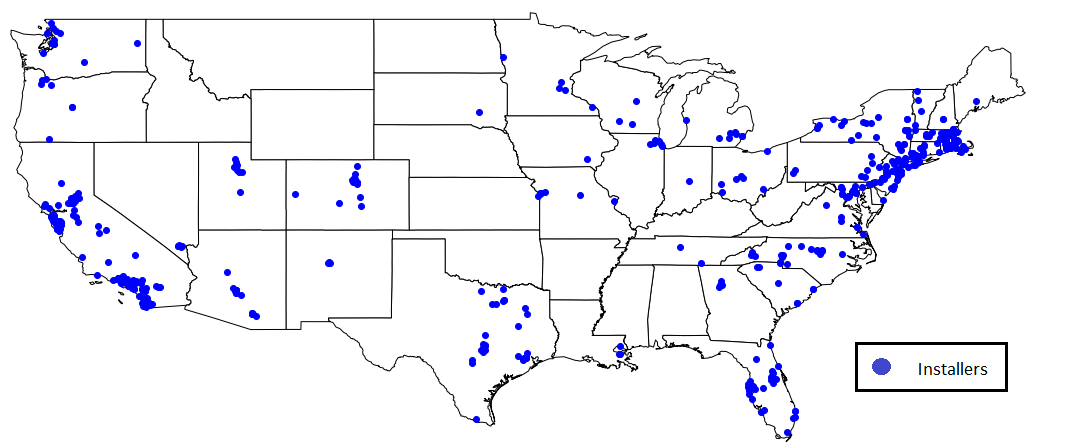
\includegraphics[width=0.7\linewidth]{national_installers}
	\caption{All Installers}
	\label{fig:nationalinstallers}
\end{figure}

\begin{figure}
	\centering
	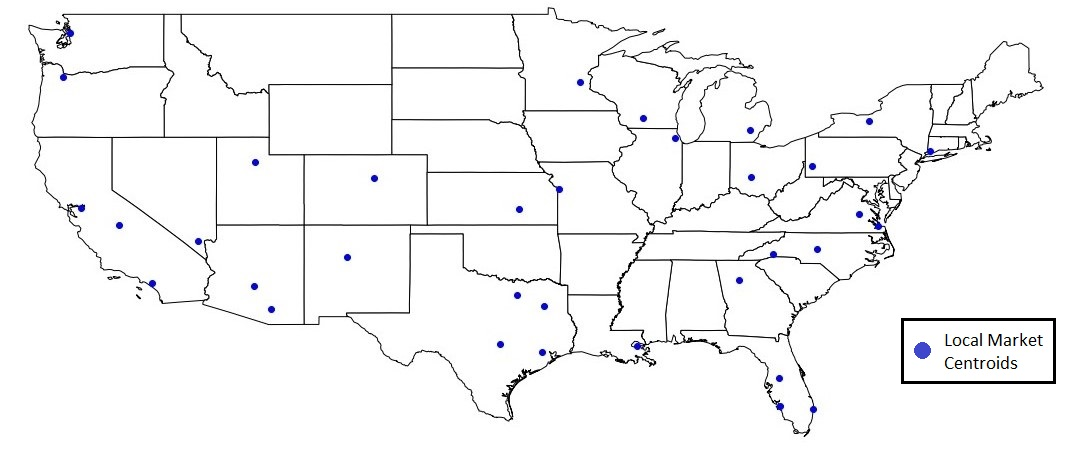
\includegraphics[width=0.7\linewidth]{markets}
	\caption{Local Market Centroids}
	\label{fig:markets}
\end{figure}

\begin{figure}
	\centering
	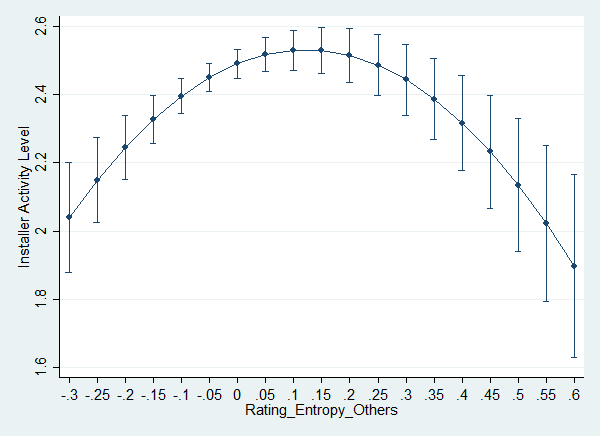
\includegraphics[width=0.7\linewidth]{marginsplot_entothers}
	\caption{Marginal Impact of Entropy of Reviews}
	\label{fig:markets}
\end{figure}  

\end{APPENDIX}
% Appendix here
% Options are (1) APPENDIX (with or without general title) or
%             (2) APPENDICES (if it has more than one unrelated sections)
% Outcomment the appropriate case if necessary
%
% \begin{APPENDIX}{<Title of the Appendix>}
% \end{APPENDIX}
%
%   or
%
% \begin{APPENDICES}
% \section{<Title of Section A>}
% \section{<Title of Section B>}
% etc
% \end{APPENDICES}


% Acknowledgments here
\ACKNOWLEDGMENT{The authors gratefully acknowledge the existence of
the Journal of Irreproducible Results and the support of the Society
for the Preservation of Inane Research.}


% References here (outcomment the appropriate case)

% CASE 1: BiBTeX used to constantly update the references
%   (while the paper is being written).
%\bibliographystyle{informs2014} % outcomment this and next line in Case 1
%\bibliography{<your bib file(s)>} % if more than one, comma separated

% CASE 2: BiBTeX used to generate mypaper.bbl (to be further fine tuned)
%\input{mypaper.bbl} % outcomment this line in Case 2

%If you don't use BiBTex, you can manually itemize references as shown below.

\bibliographystyle{nonumber}

 
%%%%%%%%%%%%%%%%%
\end{document}
%%%%%%%%%%%%%%%%%

